\documentclass[1p]{elsarticle_modified}
%\bibliographystyle{elsarticle-num}

%\usepackage[colorlinks]{hyperref}
%\usepackage{abbrmath_seonhwa} %\Abb, \Ascr, \Acal ,\Abf, \Afrak
\usepackage{amsfonts}
\usepackage{amssymb}
\usepackage{amsmath}
\usepackage{amsthm}
\usepackage{scalefnt}
\usepackage{amsbsy}
\usepackage{kotex}
\usepackage{caption}
\usepackage{subfig}
\usepackage{color}
\usepackage{graphicx}
\usepackage{xcolor} %% white, black, red, green, blue, cyan, magenta, yellow
\usepackage{float}
\usepackage{setspace}
\usepackage{hyperref}

\usepackage{tikz}
\usetikzlibrary{arrows}

\usepackage{multirow}
\usepackage{array} % fixed length table
\usepackage{hhline}

%%%%%%%%%%%%%%%%%%%%%
\makeatletter
\renewcommand*\env@matrix[1][\arraystretch]{%
	\edef\arraystretch{#1}%
	\hskip -\arraycolsep
	\let\@ifnextchar\new@ifnextchar
	\array{*\c@MaxMatrixCols c}}
\makeatother %https://tex.stackexchange.com/questions/14071/how-can-i-increase-the-line-spacing-in-a-matrix
%%%%%%%%%%%%%%%

\usepackage[normalem]{ulem}

\newcommand{\msout}[1]{\ifmmode\text{\sout{\ensuremath{#1}}}\else\sout{#1}\fi}
%SOURCE: \msout is \stkout macro in https://tex.stackexchange.com/questions/20609/strikeout-in-math-mode

\newcommand{\cancel}[1]{
	\ifmmode
	{\color{red}\msout{#1}}
	\else
	{\color{red}\sout{#1}}
	\fi
}

\newcommand{\add}[1]{
	{\color{blue}\uwave{#1}}
}

\newcommand{\replace}[2]{
	\ifmmode
	{\color{red}\msout{#1}}{\color{blue}\uwave{#2}}
	\else
	{\color{red}\sout{#1}}{\color{blue}\uwave{#2}}
	\fi
}

\newcommand{\Sol}{\mathcal{S}} %segment
\newcommand{\D}{D} %diagram
\newcommand{\A}{\mathcal{A}} %arc


%%%%%%%%%%%%%%%%%%%%%%%%%%%%%5 test

\def\sl{\operatorname{\textup{SL}}(2,\Cbb)}
\def\psl{\operatorname{\textup{PSL}}(2,\Cbb)}
\def\quan{\mkern 1mu \triangleright \mkern 1mu}

\theoremstyle{definition}
\newtheorem{thm}{Theorem}[section]
\newtheorem{prop}[thm]{Proposition}
\newtheorem{lem}[thm]{Lemma}
\newtheorem{ques}[thm]{Question}
\newtheorem{cor}[thm]{Corollary}
\newtheorem{defn}[thm]{Definition}
\newtheorem{exam}[thm]{Example}
\newtheorem{rmk}[thm]{Remark}
\newtheorem{alg}[thm]{Algorithm}

\newcommand{\I}{\sqrt{-1}}
\begin{document}

%\begin{frontmatter}
%
%\title{Boundary parabolic representations of knots up to 8 crossings}
%
%%% Group authors per affiliation:
%\author{Yunhi Cho} 
%\address{Department of Mathematics, University of Seoul, Seoul, Korea}
%\ead{yhcho@uos.ac.kr}
%
%
%\author{Seonhwa Kim} %\fnref{s_kim}}
%\address{Center for Geometry and Physics, Institute for Basic Science, Pohang, 37673, Korea}
%\ead{ryeona17@ibs.re.kr}
%
%\author{Hyuk Kim}
%\address{Department of Mathematical Sciences, Seoul National University, Seoul 08826, Korea}
%\ead{hyukkim@snu.ac.kr}
%
%\author{Seokbeom Yoon}
%\address{Department of Mathematical Sciences, Seoul National University, Seoul, 08826,  Korea}
%\ead{sbyoon15@snu.ac.kr}
%
%\begin{abstract}
%We find all boundary parabolic representation of knots up to 8 crossings.
%
%\end{abstract}
%\begin{keyword}
%    \MSC[2010] 57M25 
%\end{keyword}
%
%\end{frontmatter}

%\linenumbers
%\tableofcontents
%
\newcommand\colored[1]{\textcolor{white}{\rule[-0.35ex]{0.8em}{1.4ex}}\kern-0.8em\color{red} #1}%
%\newcommand\colored[1]{\textcolor{white}{ #1}\kern-2.17ex	\textcolor{white}{ #1}\kern-1.81ex	\textcolor{white}{ #1}\kern-2.15ex\color{red}#1	}

{\Large $\underline{12n_{0762}~(K12n_{0762})}$}

\setlength{\tabcolsep}{10pt}
\renewcommand{\arraystretch}{1.6}
\vspace{1cm}\begin{tabular}{m{100pt}>{\centering\arraybackslash}m{274pt}}
\multirow{5}{120pt}{
	\centering
	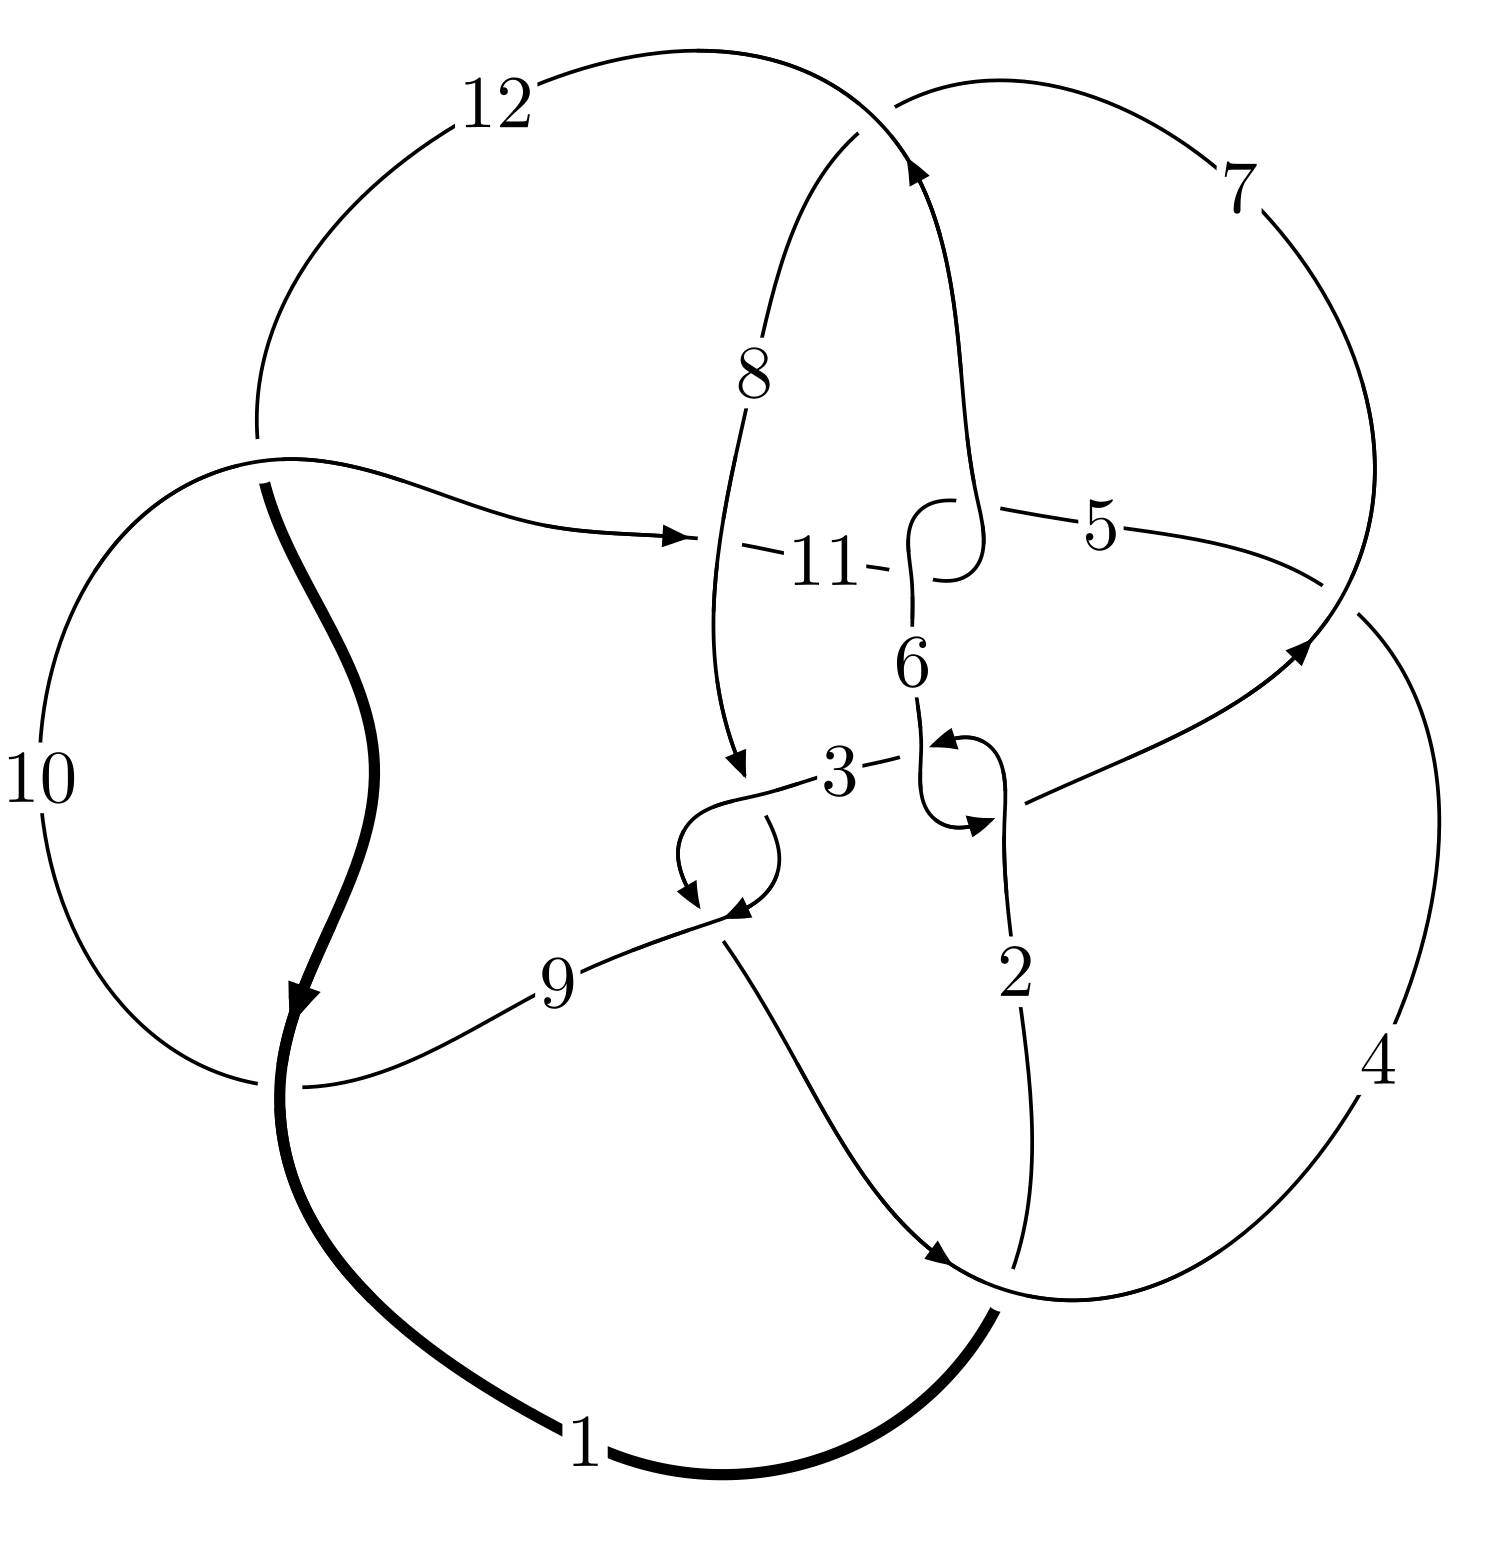
\includegraphics[width=112pt]{../../../GIT/diagram.site/Diagrams/png/2851_12n_0762.png}\\
\ \ \ A knot diagram\footnotemark}&
\allowdisplaybreaks
\textbf{Linearized knot diagam} \\
\cline{2-2}
 &
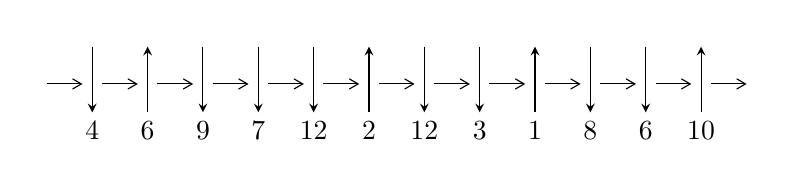
\begin{tikzpicture}[x=20pt, y=17pt]
	% nodes
	\node (C0) at (0, 0) {};
	\node (C1) at (1, 0) {};
	\node (C1U) at (1, +1) {};
	\node (C1D) at (1, -1) {4};

	\node (C2) at (2, 0) {};
	\node (C2U) at (2, +1) {};
	\node (C2D) at (2, -1) {6};

	\node (C3) at (3, 0) {};
	\node (C3U) at (3, +1) {};
	\node (C3D) at (3, -1) {9};

	\node (C4) at (4, 0) {};
	\node (C4U) at (4, +1) {};
	\node (C4D) at (4, -1) {7};

	\node (C5) at (5, 0) {};
	\node (C5U) at (5, +1) {};
	\node (C5D) at (5, -1) {12};

	\node (C6) at (6, 0) {};
	\node (C6U) at (6, +1) {};
	\node (C6D) at (6, -1) {2};

	\node (C7) at (7, 0) {};
	\node (C7U) at (7, +1) {};
	\node (C7D) at (7, -1) {12};

	\node (C8) at (8, 0) {};
	\node (C8U) at (8, +1) {};
	\node (C8D) at (8, -1) {3};

	\node (C9) at (9, 0) {};
	\node (C9U) at (9, +1) {};
	\node (C9D) at (9, -1) {1};

	\node (C10) at (10, 0) {};
	\node (C10U) at (10, +1) {};
	\node (C10D) at (10, -1) {8};

	\node (C11) at (11, 0) {};
	\node (C11U) at (11, +1) {};
	\node (C11D) at (11, -1) {6};

	\node (C12) at (12, 0) {};
	\node (C12U) at (12, +1) {};
	\node (C12D) at (12, -1) {10};
	\node (C13) at (13, 0) {};

	% arrows
	\draw[->,>={angle 60}]
	(C0) edge (C1) (C1) edge (C2) (C2) edge (C3) (C3) edge (C4) (C4) edge (C5) (C5) edge (C6) (C6) edge (C7) (C7) edge (C8) (C8) edge (C9) (C9) edge (C10) (C10) edge (C11) (C11) edge (C12) (C12) edge (C13) ;	\draw[->,>=stealth]
	(C1U) edge (C1D) (C2D) edge (C2U) (C3U) edge (C3D) (C4U) edge (C4D) (C5U) edge (C5D) (C6D) edge (C6U) (C7U) edge (C7D) (C8U) edge (C8D) (C9D) edge (C9U) (C10U) edge (C10D) (C11U) edge (C11D) (C12D) edge (C12U) ;
	\end{tikzpicture} \\
\hhline{~~} \\& 
\textbf{Solving Sequence} \\ \cline{2-2} 
 &
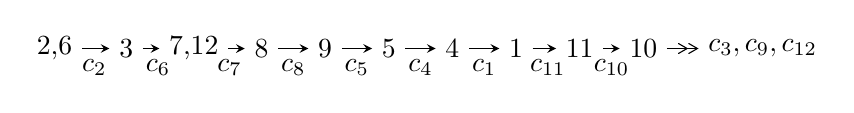
\begin{tikzpicture}[x=23pt, y=7pt]
	% node
	\node (A0) at (-1/8, 0) {2,6};
	\node (A1) at (1, 0) {3};
	\node (A2) at (33/16, 0) {7,12};
	\node (A3) at (25/8, 0) {8};
	\node (A4) at (33/8, 0) {9};
	\node (A5) at (41/8, 0) {5};
	\node (A6) at (49/8, 0) {4};
	\node (A7) at (57/8, 0) {1};
	\node (A8) at (65/8, 0) {11};
	\node (A9) at (73/8, 0) {10};
	\node (C1) at (1/2, -1) {$c_{2}$};
	\node (C2) at (3/2, -1) {$c_{6}$};
	\node (C3) at (21/8, -1) {$c_{7}$};
	\node (C4) at (29/8, -1) {$c_{8}$};
	\node (C5) at (37/8, -1) {$c_{5}$};
	\node (C6) at (45/8, -1) {$c_{4}$};
	\node (C7) at (53/8, -1) {$c_{1}$};
	\node (C8) at (61/8, -1) {$c_{11}$};
	\node (C9) at (69/8, -1) {$c_{10}$};
	\node (A10) at (11, 0) {$c_{3},c_{9},c_{12}$};

	% edge
	\draw[->,>=stealth]	
	(A0) edge (A1) (A1) edge (A2) (A2) edge (A3) (A3) edge (A4) (A4) edge (A5) (A5) edge (A6) (A6) edge (A7) (A7) edge (A8) (A8) edge (A9) ;
	\draw[->>,>={angle 60}]	
	(A9) edge (A10);
\end{tikzpicture} \\ 

\end{tabular} \\

\footnotetext{
The image of knot diagram is generated by the software ``\textbf{Draw programme}" developed by Andrew Bartholomew(\url{http://www.layer8.co.uk/maths/draw/index.htm\#Running-draw}), where we modified some parts for our purpose(\url{https://github.com/CATsTAILs/LinksPainter}).
}\phantom \\ \newline 
\centering \textbf{Ideals for irreducible components\footnotemark of $X_{\text{par}}$} 
 
\begin{align*}
I^u_{1}&=\langle 
-6.39438\times10^{155} u^{61}-1.83142\times10^{156} u^{60}+\cdots+1.27661\times10^{155} b+4.88446\times10^{156},\\
\phantom{I^u_{1}}&\phantom{= \langle  }-4.08969\times10^{156} u^{61}-1.17222\times10^{157} u^{60}+\cdots+1.27661\times10^{155} a+3.11795\times10^{157},\\
\phantom{I^u_{1}}&\phantom{= \langle  }u^{62}+3 u^{61}+\cdots-18 u-1\rangle \\
I^u_{2}&=\langle 
-4390048992 u^{27}+17294455334 u^{26}+\cdots+1052877967 b-16499967912,\\
\phantom{I^u_{2}}&\phantom{= \langle  }-1778777089 u^{27}+10103913125 u^{26}+\cdots+1052877967 a-14753500781,\\
\phantom{I^u_{2}}&\phantom{= \langle  }u^{28}-2 u^{27}+\cdots-3 u-1\rangle \\
\\
\end{align*}
\raggedright * 2 irreducible components of $\dim_{\mathbb{C}}=0$, with total 90 representations.\\
\footnotetext{All coefficients of polynomials are rational numbers. But the coefficients are sometimes approximated in decimal forms when there is not enough margin.}
\newpage
\renewcommand{\arraystretch}{1}
\centering \section*{I. $I^u_{1}= \langle -6.39\times10^{155} u^{61}-1.83\times10^{156} u^{60}+\cdots+1.28\times10^{155} b+4.88\times10^{156},\;-4.09\times10^{156} u^{61}-1.17\times10^{157} u^{60}+\cdots+1.28\times10^{155} a+3.12\times10^{157},\;u^{62}+3 u^{61}+\cdots-18 u-1 \rangle$}
\flushleft \textbf{(i) Arc colorings}\\
\begin{tabular}{m{7pt} m{180pt} m{7pt} m{180pt} }
\flushright $a_{2}=$&$\begin{pmatrix}1\\0\end{pmatrix}$ \\
\flushright $a_{6}=$&$\begin{pmatrix}0\\u\end{pmatrix}$ \\
\flushright $a_{3}=$&$\begin{pmatrix}1\\- u^2\end{pmatrix}$ \\
\flushright $a_{7}=$&$\begin{pmatrix}u\\u\end{pmatrix}$ \\
\flushright $a_{12}=$&$\begin{pmatrix}32.0357 u^{61}+91.8228 u^{60}+\cdots-2497.42 u-244.237\\5.00889 u^{61}+14.3460 u^{60}+\cdots-387.238 u-38.2613\end{pmatrix}$ \\
\flushright $a_{8}=$&$\begin{pmatrix}-5.65842 u^{61}-16.2812 u^{60}+\cdots+456.306 u+40.1573\\3.01761 u^{61}+8.66285 u^{60}+\cdots-242.152 u-24.6253\end{pmatrix}$ \\
\flushright $a_{9}=$&$\begin{pmatrix}-8.58616 u^{61}-24.6845 u^{60}+\cdots+691.623 u+64.0885\\3.06626 u^{61}+8.80184 u^{60}+\cdots-246.062 u-25.0051\end{pmatrix}$ \\
\flushright $a_{5}=$&$\begin{pmatrix}1.10750 u^{61}+3.21521 u^{60}+\cdots-87.7707 u-3.39247\\-4.55092 u^{61}-13.0660 u^{60}+\cdots+368.535 u+36.7648\end{pmatrix}$ \\
\flushright $a_{4}=$&$\begin{pmatrix}1.01763 u^{61}+2.95572 u^{60}+\cdots-80.9356 u-2.69839\\-4.64079 u^{61}-13.3255 u^{60}+\cdots+375.370 u+37.4589\end{pmatrix}$ \\
\flushright $a_{1}=$&$\begin{pmatrix}14.0757 u^{61}+40.4062 u^{60}+\cdots-1167.51 u-118.139\\3.44249 u^{61}+9.89638 u^{60}+\cdots-294.292 u-28.6685\end{pmatrix}$ \\
\flushright $a_{11}=$&$\begin{pmatrix}32.0357 u^{61}+91.8228 u^{60}+\cdots-2497.42 u-244.237\\4.46323 u^{61}+12.7861 u^{60}+\cdots-342.159 u-33.9771\end{pmatrix}$ \\
\flushright $a_{10}=$&$\begin{pmatrix}18.5714 u^{61}+53.2721 u^{60}+\cdots-1400.80 u-141.560\\-0.0553237 u^{61}-0.161959 u^{60}+\cdots+11.9855 u-0.335246\end{pmatrix}$\\&\end{tabular}
\flushleft \textbf{(ii) Obstruction class $= -1$}\\~\\
\flushleft \textbf{(iii) Cusp Shapes $= -5.41881 u^{61}-15.7513 u^{60}+\cdots+462.106 u+47.0844$}\\~\\
\newpage\renewcommand{\arraystretch}{1}
\flushleft \textbf{(iv) u-Polynomials at the component}\newline \\
\begin{tabular}{m{50pt}|m{274pt}}
Crossings & \hspace{64pt}u-Polynomials at each crossing \\
\hline $$\begin{aligned}c_{1}\end{aligned}$$&$\begin{aligned}
&u^{62}-8 u^{61}+\cdots-14573 u-2354
\end{aligned}$\\
\hline $$\begin{aligned}c_{2},c_{6}\end{aligned}$$&$\begin{aligned}
&u^{62}-3 u^{61}+\cdots+18 u-1
\end{aligned}$\\
\hline $$\begin{aligned}c_{3},c_{8}\end{aligned}$$&$\begin{aligned}
&u^{62}- u^{61}+\cdots-1064 u+127
\end{aligned}$\\
\hline $$\begin{aligned}c_{4}\end{aligned}$$&$\begin{aligned}
&u^{62}-7 u^{61}+\cdots+2345 u-631
\end{aligned}$\\
\hline $$\begin{aligned}c_{5},c_{11}\end{aligned}$$&$\begin{aligned}
&u^{62}- u^{61}+\cdots-67775 u+24008
\end{aligned}$\\
\hline $$\begin{aligned}c_{7}\end{aligned}$$&$\begin{aligned}
&u^{62}+3 u^{61}+\cdots-11203 u+18287
\end{aligned}$\\
\hline $$\begin{aligned}c_{9},c_{12}\end{aligned}$$&$\begin{aligned}
&u^{62}+5 u^{61}+\cdots+7 u+1
\end{aligned}$\\
\hline $$\begin{aligned}c_{10}\end{aligned}$$&$\begin{aligned}
&u^{62}-13 u^{61}+\cdots+690763 u-71359
\end{aligned}$\\
\hline
\end{tabular}\\~\\
\newpage\renewcommand{\arraystretch}{1}
\flushleft \textbf{(v) Riley Polynomials at the component}\newline \\
\begin{tabular}{m{50pt}|m{274pt}}
Crossings & \hspace{64pt}Riley Polynomials at each crossing \\
\hline $$\begin{aligned}c_{1}\end{aligned}$$&$\begin{aligned}
&y^{62}-30 y^{61}+\cdots+87051763 y+5541316
\end{aligned}$\\
\hline $$\begin{aligned}c_{2},c_{6}\end{aligned}$$&$\begin{aligned}
&y^{62}+59 y^{61}+\cdots-98 y+1
\end{aligned}$\\
\hline $$\begin{aligned}c_{3},c_{8}\end{aligned}$$&$\begin{aligned}
&y^{62}-57 y^{61}+\cdots-252240 y+16129
\end{aligned}$\\
\hline $$\begin{aligned}c_{4}\end{aligned}$$&$\begin{aligned}
&y^{62}-95 y^{61}+\cdots-19707883 y+398161
\end{aligned}$\\
\hline $$\begin{aligned}c_{5},c_{11}\end{aligned}$$&$\begin{aligned}
&y^{62}-99 y^{61}+\cdots-7503268241 y+576384064
\end{aligned}$\\
\hline $$\begin{aligned}c_{7}\end{aligned}$$&$\begin{aligned}
&y^{62}-89 y^{61}+\cdots-6246385553 y+334414369
\end{aligned}$\\
\hline $$\begin{aligned}c_{9},c_{12}\end{aligned}$$&$\begin{aligned}
&y^{62}+51 y^{61}+\cdots-37 y+1
\end{aligned}$\\
\hline $$\begin{aligned}c_{10}\end{aligned}$$&$\begin{aligned}
&y^{62}-81 y^{61}+\cdots+2924033206473 y+5092106881
\end{aligned}$\\
\hline
\end{tabular}\\~\\
\newpage\flushleft \textbf{(vi) Complex Volumes and Cusp Shapes}
$$\begin{array}{c|c|c}  
\text{Solutions to }I^u_{1}& \I (\text{vol} + \sqrt{-1}CS) & \text{Cusp shape}\\
 \hline 
\begin{aligned}
u &= -0.333052 + 0.944555 I \\
a &= \phantom{-}0.389031 - 0.384339 I \\
b &= -0.154212 - 0.620844 I\end{aligned}
 & -0.62353 - 1.46430 I & \phantom{-0.000000 } 0 \\ \hline\begin{aligned}
u &= -0.333052 - 0.944555 I \\
a &= \phantom{-}0.389031 + 0.384339 I \\
b &= -0.154212 + 0.620844 I\end{aligned}
 & -0.62353 + 1.46430 I & \phantom{-0.000000 } 0 \\ \hline\begin{aligned}
u &= \phantom{-}0.832713 + 0.485235 I \\
a &= -0.254095 + 0.534839 I \\
b &= -0.07870 + 1.70723 I\end{aligned}
 & \phantom{-}0.80228 + 3.34364 I & \phantom{-0.000000 } 0 \\ \hline\begin{aligned}
u &= \phantom{-}0.832713 - 0.485235 I \\
a &= -0.254095 - 0.534839 I \\
b &= -0.07870 - 1.70723 I\end{aligned}
 & \phantom{-}0.80228 - 3.34364 I & \phantom{-0.000000 } 0 \\ \hline\begin{aligned}
u &= -0.589027 + 0.853031 I \\
a &= \phantom{-}0.727906 + 0.227126 I \\
b &= \phantom{-}0.309790 - 0.219659 I\end{aligned}
 & -0.90701 - 2.10996 I & \phantom{-0.000000 } 0 \\ \hline\begin{aligned}
u &= -0.589027 - 0.853031 I \\
a &= \phantom{-}0.727906 - 0.227126 I \\
b &= \phantom{-}0.309790 + 0.219659 I\end{aligned}
 & -0.90701 + 2.10996 I & \phantom{-0.000000 } 0 \\ \hline\begin{aligned}
u &= -0.183155 + 1.090710 I \\
a &= -0.870044 + 0.673371 I \\
b &= -0.590651 + 1.128490 I\end{aligned}
 & -4.41723 - 3.27563 I & \phantom{-0.000000 } 0 \\ \hline\begin{aligned}
u &= -0.183155 - 1.090710 I \\
a &= -0.870044 - 0.673371 I \\
b &= -0.590651 - 1.128490 I\end{aligned}
 & -4.41723 + 3.27563 I & \phantom{-0.000000 } 0 \\ \hline\begin{aligned}
u &= -0.958678 + 0.626520 I \\
a &= \phantom{-}0.093398 - 0.975017 I \\
b &= -0.24619 - 1.53004 I\end{aligned}
 & \phantom{-}0.14869 - 2.80498 I & \phantom{-0.000000 } 0 \\ \hline\begin{aligned}
u &= -0.958678 - 0.626520 I \\
a &= \phantom{-}0.093398 + 0.975017 I \\
b &= -0.24619 + 1.53004 I\end{aligned}
 & \phantom{-}0.14869 + 2.80498 I & \phantom{-0.000000 } 0\\
 \hline 
 \end{array}$$\newpage$$\begin{array}{c|c|c}  
\text{Solutions to }I^u_{1}& \I (\text{vol} + \sqrt{-1}CS) & \text{Cusp shape}\\
 \hline 
\begin{aligned}
u &= \phantom{-}0.807646 + 0.092651 I \\
a &= -0.386650 + 0.557445 I \\
b &= \phantom{-}0.224777 - 0.223097 I\end{aligned}
 & -5.34851 - 2.44220 I & \phantom{-0.000000 } 0 \\ \hline\begin{aligned}
u &= \phantom{-}0.807646 - 0.092651 I \\
a &= -0.386650 - 0.557445 I \\
b &= \phantom{-}0.224777 + 0.223097 I\end{aligned}
 & -5.34851 + 2.44220 I & \phantom{-0.000000 } 0 \\ \hline\begin{aligned}
u &= \phantom{-}0.770858\phantom{ +0.000000I} \\
a &= \phantom{-}1.84196\phantom{ +0.000000I} \\
b &= -0.196952\phantom{ +0.000000I}\end{aligned}
 & -3.55600\phantom{ +0.000000I} & \phantom{-0.000000 } 0 \\ \hline\begin{aligned}
u &= -0.350668 + 1.211440 I \\
a &= -0.074129 + 0.331633 I \\
b &= \phantom{-}1.006790 + 0.617776 I\end{aligned}
 & -3.91833 - 0.86784 I & \phantom{-0.000000 } 0 \\ \hline\begin{aligned}
u &= -0.350668 - 1.211440 I \\
a &= -0.074129 - 0.331633 I \\
b &= \phantom{-}1.006790 - 0.617776 I\end{aligned}
 & -3.91833 + 0.86784 I & \phantom{-0.000000 } 0 \\ \hline\begin{aligned}
u &= \phantom{-}0.066377 + 0.729220 I \\
a &= \phantom{-}0.474227 - 0.548295 I \\
b &= -0.416502 - 0.022118 I\end{aligned}
 & -0.903631 - 1.036690 I & -6.98552 + 4.12911 I \\ \hline\begin{aligned}
u &= \phantom{-}0.066377 - 0.729220 I \\
a &= \phantom{-}0.474227 + 0.548295 I \\
b &= -0.416502 + 0.022118 I\end{aligned}
 & -0.903631 + 1.036690 I & -6.98552 - 4.12911 I \\ \hline\begin{aligned}
u &= \phantom{-}0.454755 + 1.195890 I \\
a &= -0.313664 + 0.218835 I \\
b &= -0.336580 + 0.566077 I\end{aligned}
 & -4.85375 + 4.25052 I & \phantom{-0.000000 } 0 \\ \hline\begin{aligned}
u &= \phantom{-}0.454755 - 1.195890 I \\
a &= -0.313664 - 0.218835 I \\
b &= -0.336580 - 0.566077 I\end{aligned}
 & -4.85375 - 4.25052 I & \phantom{-0.000000 } 0 \\ \hline\begin{aligned}
u &= \phantom{-}0.698392 + 0.177356 I \\
a &= -1.92419 + 0.75830 I \\
b &= \phantom{-}0.236377 + 0.216993 I\end{aligned}
 & -7.74561 + 4.18757 I & -4.00000 - 3.79519 I\\
 \hline 
 \end{array}$$\newpage$$\begin{array}{c|c|c}  
\text{Solutions to }I^u_{1}& \I (\text{vol} + \sqrt{-1}CS) & \text{Cusp shape}\\
 \hline 
\begin{aligned}
u &= \phantom{-}0.698392 - 0.177356 I \\
a &= -1.92419 - 0.75830 I \\
b &= \phantom{-}0.236377 - 0.216993 I\end{aligned}
 & -7.74561 - 4.18757 I & -4.00000 + 3.79519 I \\ \hline\begin{aligned}
u &= \phantom{-}0.459690 + 1.195230 I \\
a &= \phantom{-}0.548483 + 0.114412 I \\
b &= \phantom{-}0.911400 - 0.215151 I\end{aligned}
 & -8.60885 + 7.03690 I & \phantom{-0.000000 } 0 \\ \hline\begin{aligned}
u &= \phantom{-}0.459690 - 1.195230 I \\
a &= \phantom{-}0.548483 - 0.114412 I \\
b &= \phantom{-}0.911400 + 0.215151 I\end{aligned}
 & -8.60885 - 7.03690 I & \phantom{-0.000000 } 0 \\ \hline\begin{aligned}
u &= \phantom{-}0.435856 + 1.211820 I \\
a &= \phantom{-}0.098938 - 0.576576 I \\
b &= -0.278422 - 1.000790 I\end{aligned}
 & -9.25216 + 1.84332 I & \phantom{-0.000000 } 0 \\ \hline\begin{aligned}
u &= \phantom{-}0.435856 - 1.211820 I \\
a &= \phantom{-}0.098938 + 0.576576 I \\
b &= -0.278422 + 1.000790 I\end{aligned}
 & -9.25216 - 1.84332 I & \phantom{-0.000000 } 0 \\ \hline\begin{aligned}
u &= \phantom{-}0.696310\phantom{ +0.000000I} \\
a &= \phantom{-}0.539160\phantom{ +0.000000I} \\
b &= -0.210110\phantom{ +0.000000I}\end{aligned}
 & -1.50281\phantom{ +0.000000I} & -7.64330\phantom{ +0.000000I} \\ \hline\begin{aligned}
u &= \phantom{-}0.12810 + 1.44057 I \\
a &= \phantom{-}0.39257 + 1.87823 I \\
b &= \phantom{-}0.23423 + 2.96746 I\end{aligned}
 & -15.6787 + 2.6099 I & \phantom{-0.000000 } 0 \\ \hline\begin{aligned}
u &= \phantom{-}0.12810 - 1.44057 I \\
a &= \phantom{-}0.39257 - 1.87823 I \\
b &= \phantom{-}0.23423 - 2.96746 I\end{aligned}
 & -15.6787 - 2.6099 I & \phantom{-0.000000 } 0 \\ \hline\begin{aligned}
u &= \phantom{-}0.28124 + 1.49021 I \\
a &= \phantom{-}0.29340 - 1.43793 I \\
b &= \phantom{-}0.35314 - 2.63889 I\end{aligned}
 & -12.38030 - 0.46591 I & \phantom{-0.000000 } 0 \\ \hline\begin{aligned}
u &= \phantom{-}0.28124 - 1.49021 I \\
a &= \phantom{-}0.29340 + 1.43793 I \\
b &= \phantom{-}0.35314 + 2.63889 I\end{aligned}
 & -12.38030 + 0.46591 I & \phantom{-0.000000 } 0\\
 \hline 
 \end{array}$$\newpage$$\begin{array}{c|c|c}  
\text{Solutions to }I^u_{1}& \I (\text{vol} + \sqrt{-1}CS) & \text{Cusp shape}\\
 \hline 
\begin{aligned}
u &= \phantom{-}0.14213 + 1.52049 I \\
a &= -0.27464 - 1.43449 I \\
b &= \phantom{-}0.01746 - 2.61143 I\end{aligned}
 & -12.42090 + 1.93692 I & \phantom{-0.000000 } 0 \\ \hline\begin{aligned}
u &= \phantom{-}0.14213 - 1.52049 I \\
a &= -0.27464 + 1.43449 I \\
b &= \phantom{-}0.01746 + 2.61143 I\end{aligned}
 & -12.42090 - 1.93692 I & \phantom{-0.000000 } 0 \\ \hline\begin{aligned}
u &= \phantom{-}0.26991 + 1.53473 I \\
a &= -0.180066 + 1.299350 I \\
b &= -0.17141 + 2.61130 I\end{aligned}
 & -9.12418 + 3.84227 I & \phantom{-0.000000 } 0 \\ \hline\begin{aligned}
u &= \phantom{-}0.26991 - 1.53473 I \\
a &= -0.180066 - 1.299350 I \\
b &= -0.17141 - 2.61130 I\end{aligned}
 & -9.12418 - 3.84227 I & \phantom{-0.000000 } 0 \\ \hline\begin{aligned}
u &= -0.08283 + 1.56880 I \\
a &= -1.068300 - 0.728241 I \\
b &= -0.589996 - 1.278450 I\end{aligned}
 & -9.51760 + 5.08658 I & \phantom{-0.000000 } 0 \\ \hline\begin{aligned}
u &= -0.08283 - 1.56880 I \\
a &= -1.068300 + 0.728241 I \\
b &= -0.589996 + 1.278450 I\end{aligned}
 & -9.51760 - 5.08658 I & \phantom{-0.000000 } 0 \\ \hline\begin{aligned}
u &= \phantom{-}0.27775 + 1.56012 I \\
a &= \phantom{-}0.132678 - 1.236370 I \\
b &= \phantom{-}0.09558 - 2.68981 I\end{aligned}
 & -13.8317 + 7.8929 I & \phantom{-0.000000 } 0 \\ \hline\begin{aligned}
u &= \phantom{-}0.27775 - 1.56012 I \\
a &= \phantom{-}0.132678 + 1.236370 I \\
b &= \phantom{-}0.09558 + 2.68981 I\end{aligned}
 & -13.8317 - 7.8929 I & \phantom{-0.000000 } 0 \\ \hline\begin{aligned}
u &= \phantom{-}0.15046 + 1.60424 I \\
a &= \phantom{-}0.160295 + 1.146520 I \\
b &= -0.31811 + 2.51871 I\end{aligned}
 & -17.6021 + 1.1585 I & \phantom{-0.000000 } 0 \\ \hline\begin{aligned}
u &= \phantom{-}0.15046 - 1.60424 I \\
a &= \phantom{-}0.160295 - 1.146520 I \\
b &= -0.31811 - 2.51871 I\end{aligned}
 & -17.6021 - 1.1585 I & \phantom{-0.000000 } 0\\
 \hline 
 \end{array}$$\newpage$$\begin{array}{c|c|c}  
\text{Solutions to }I^u_{1}& \I (\text{vol} + \sqrt{-1}CS) & \text{Cusp shape}\\
 \hline 
\begin{aligned}
u &= \phantom{-}0.341402 + 0.171738 I \\
a &= \phantom{-}4.13096 - 1.61392 I \\
b &= \phantom{-}0.675184 - 0.592840 I\end{aligned}
 & -11.05090 - 0.90973 I & -10.78531 - 1.39456 I \\ \hline\begin{aligned}
u &= \phantom{-}0.341402 - 0.171738 I \\
a &= \phantom{-}4.13096 + 1.61392 I \\
b &= \phantom{-}0.675184 + 0.592840 I\end{aligned}
 & -11.05090 + 0.90973 I & -10.78531 + 1.39456 I \\ \hline\begin{aligned}
u &= \phantom{-}0.03842 + 1.63568 I \\
a &= -0.527691 - 0.462807 I \\
b &= \phantom{-}0.451791 - 1.092900 I\end{aligned}
 & -10.48550 - 5.71222 I & \phantom{-0.000000 } 0 \\ \hline\begin{aligned}
u &= \phantom{-}0.03842 - 1.63568 I \\
a &= -0.527691 + 0.462807 I \\
b &= \phantom{-}0.451791 + 1.092900 I\end{aligned}
 & -10.48550 + 5.71222 I & \phantom{-0.000000 } 0 \\ \hline\begin{aligned}
u &= \phantom{-}0.359374\phantom{ +0.000000I} \\
a &= -4.34971\phantom{ +0.000000I} \\
b &= -0.676883\phantom{ +0.000000I}\end{aligned}
 & -6.85123\phantom{ +0.000000I} & -16.8270\phantom{ +0.000000I} \\ \hline\begin{aligned}
u &= -1.63565 + 0.23135 I \\
a &= -1.293770 - 0.085038 I \\
b &= -0.0375020 + 0.0652272 I\end{aligned}
 & -14.1359 - 7.0273 I & \phantom{-0.000000 } 0 \\ \hline\begin{aligned}
u &= -1.63565 - 0.23135 I \\
a &= -1.293770 + 0.085038 I \\
b &= -0.0375020 - 0.0652272 I\end{aligned}
 & -14.1359 + 7.0273 I & \phantom{-0.000000 } 0 \\ \hline\begin{aligned}
u &= -0.02899 + 1.68061 I \\
a &= \phantom{-}0.815326 + 0.498354 I \\
b &= \phantom{-}0.070018 + 1.005780 I\end{aligned}
 & -5.54238 - 0.38545 I & \phantom{-0.000000 } 0 \\ \hline\begin{aligned}
u &= -0.02899 - 1.68061 I \\
a &= \phantom{-}0.815326 - 0.498354 I \\
b &= \phantom{-}0.070018 - 1.005780 I\end{aligned}
 & -5.54238 + 0.38545 I & \phantom{-0.000000 } 0 \\ \hline\begin{aligned}
u &= -0.280510 + 0.151518 I \\
a &= -0.50395 - 2.20616 I \\
b &= -0.683528 - 0.071725 I\end{aligned}
 & -0.97360 - 1.69901 I & -2.82413 + 3.98750 I\\
 \hline 
 \end{array}$$\newpage$$\begin{array}{c|c|c}  
\text{Solutions to }I^u_{1}& \I (\text{vol} + \sqrt{-1}CS) & \text{Cusp shape}\\
 \hline 
\begin{aligned}
u &= -0.280510 - 0.151518 I \\
a &= -0.50395 + 2.20616 I \\
b &= -0.683528 + 0.071725 I\end{aligned}
 & -0.97360 + 1.69901 I & -2.82413 - 3.98750 I \\ \hline\begin{aligned}
u &= -0.63741 + 1.66286 I \\
a &= \phantom{-}0.172192 + 1.286190 I \\
b &= \phantom{-}0.29163 + 2.50361 I\end{aligned}
 & \phantom{-}19.3723 - 14.9543 I & \phantom{-0.000000 } 0 \\ \hline\begin{aligned}
u &= -0.63741 - 1.66286 I \\
a &= \phantom{-}0.172192 - 1.286190 I \\
b &= \phantom{-}0.29163 - 2.50361 I\end{aligned}
 & \phantom{-}19.3723 + 14.9543 I & \phantom{-0.000000 } 0 \\ \hline\begin{aligned}
u &= -1.82775\phantom{ +0.000000I} \\
a &= \phantom{-}1.25873\phantom{ +0.000000I} \\
b &= \phantom{-}0.0527036\phantom{ +0.000000I}\end{aligned}
 & -9.14724\phantom{ +0.000000I} & \phantom{-0.000000 } 0 \\ \hline\begin{aligned}
u &= -0.1296520 + 0.0012514 I \\
a &= -0.05922 - 4.98520 I \\
b &= \phantom{-}1.113010 - 0.819545 I\end{aligned}
 & \phantom{-}1.23431 - 1.93321 I & \phantom{-}3.80958 + 0.69705 I \\ \hline\begin{aligned}
u &= -0.1296520 - 0.0012514 I \\
a &= -0.05922 + 4.98520 I \\
b &= \phantom{-}1.113010 + 0.819545 I\end{aligned}
 & \phantom{-}1.23431 + 1.93321 I & \phantom{-}3.80958 - 0.69705 I \\ \hline\begin{aligned}
u &= -0.0707850 + 0.0951134 I \\
a &= -3.35295 + 6.50987 I \\
b &= -1.65303 + 0.74429 I\end{aligned}
 & -3.99047 - 6.24706 I & -0.93942 + 7.90678 I \\ \hline\begin{aligned}
u &= -0.0707850 - 0.0951134 I \\
a &= -3.35295 - 6.50987 I \\
b &= -1.65303 - 0.74429 I\end{aligned}
 & -3.99047 + 6.24706 I & -0.93942 - 7.90678 I \\ \hline\begin{aligned}
u &= -0.70822 + 1.75594 I \\
a &= -0.122804 - 1.218420 I \\
b &= -0.26978 - 2.37851 I\end{aligned}
 & -14.8352 - 9.0166 I & \phantom{-0.000000 } 0 \\ \hline\begin{aligned}
u &= -0.70822 - 1.75594 I \\
a &= -0.122804 + 1.218420 I \\
b &= -0.26978 + 2.37851 I\end{aligned}
 & -14.8352 + 9.0166 I & \phantom{-0.000000 } 0\\
 \hline 
 \end{array}$$\newpage$$\begin{array}{c|c|c}  
\text{Solutions to }I^u_{1}& \I (\text{vol} + \sqrt{-1}CS) & \text{Cusp shape}\\
 \hline 
\begin{aligned}
u &= -0.89562 + 1.71883 I \\
a &= \phantom{-}0.131696 + 1.125940 I \\
b &= \phantom{-}0.34909 + 2.24166 I\end{aligned}
 & -18.4977 - 2.0999 I & \phantom{-0.000000 } 0 \\ \hline\begin{aligned}
u &= -0.89562 - 1.71883 I \\
a &= \phantom{-}0.131696 - 1.125940 I \\
b &= \phantom{-}0.34909 - 2.24166 I\end{aligned}
 & -18.4977 + 2.0999 I & \phantom{-0.000000 } 0\\
 \hline 
 \end{array}$$\newpage\newpage\renewcommand{\arraystretch}{1}
\centering \section*{II. $I^u_{2}= \langle -4.39\times10^{9} u^{27}+1.73\times10^{10} u^{26}+\cdots+1.05\times10^{9} b-1.65\times10^{10},\;-1.78\times10^{9} u^{27}+1.01\times10^{10} u^{26}+\cdots+1.05\times10^{9} a-1.48\times10^{10},\;u^{28}-2 u^{27}+\cdots-3 u-1 \rangle$}
\flushleft \textbf{(i) Arc colorings}\\
\begin{tabular}{m{7pt} m{180pt} m{7pt} m{180pt} }
\flushright $a_{2}=$&$\begin{pmatrix}1\\0\end{pmatrix}$ \\
\flushright $a_{6}=$&$\begin{pmatrix}0\\u\end{pmatrix}$ \\
\flushright $a_{3}=$&$\begin{pmatrix}1\\- u^2\end{pmatrix}$ \\
\flushright $a_{7}=$&$\begin{pmatrix}u\\u\end{pmatrix}$ \\
\flushright $a_{12}=$&$\begin{pmatrix}1.68944 u^{27}-9.59647 u^{26}+\cdots+24.1792 u+14.0125\\4.16957 u^{27}-16.4259 u^{26}+\cdots+32.1745 u+15.6713\end{pmatrix}$ \\
\flushright $a_{8}=$&$\begin{pmatrix}-2.24104 u^{27}+7.12886 u^{26}+\cdots-3.77423 u-5.73930\\2.94974 u^{27}-7.15613 u^{26}+\cdots-15.1617 u-2.88782\end{pmatrix}$ \\
\flushright $a_{9}=$&$\begin{pmatrix}-4.88782 u^{27}+13.7254 u^{26}+\cdots+5.68818 u-5.49827\\2.90344 u^{27}-6.26923 u^{26}+\cdots-16.4238 u-4.19078\end{pmatrix}$ \\
\flushright $a_{5}=$&$\begin{pmatrix}-0.706864 u^{27}+0.0240004 u^{26}+\cdots+5.39279 u+5.52854\\-2.94790 u^{27}+7.15286 u^{26}+\cdots+1.61856 u-0.210764\end{pmatrix}$ \\
\flushright $a_{4}=$&$\begin{pmatrix}-1.00982 u^{27}+0.583605 u^{26}+\cdots+11.0921 u+8.17533\\-3.25085 u^{27}+7.71247 u^{26}+\cdots+7.31789 u+2.43602\end{pmatrix}$ \\
\flushright $a_{1}=$&$\begin{pmatrix}-0.0543874 u^{27}+4.91254 u^{26}+\cdots-27.6210 u-16.4249\\-0.355447 u^{27}-3.74364 u^{26}+\cdots+2.08328 u-0.417512\end{pmatrix}$ \\
\flushright $a_{11}=$&$\begin{pmatrix}1.68944 u^{27}-9.59647 u^{26}+\cdots+24.1792 u+14.0125\\2.50358 u^{27}-14.8480 u^{26}+\cdots+49.1378 u+21.8889\end{pmatrix}$ \\
\flushright $a_{10}=$&$\begin{pmatrix}6.69021 u^{27}-18.1519 u^{26}+\cdots-16.4160 u-3.40215\\0.584244 u^{27}-13.8628 u^{26}+\cdots+64.1728 u+26.2558\end{pmatrix}$\\&\end{tabular}
\flushleft \textbf{(ii) Obstruction class $= 1$}\\~\\
\flushleft \textbf{(iii) Cusp Shapes $= -\frac{2679606931}{1052877967} u^{27}-\frac{15977495031}{1052877967} u^{26}+\cdots+\frac{130752365383}{1052877967} u+\frac{40877254048}{1052877967}$}\\~\\
\newpage\renewcommand{\arraystretch}{1}
\flushleft \textbf{(iv) u-Polynomials at the component}\newline \\
\begin{tabular}{m{50pt}|m{274pt}}
Crossings & \hspace{64pt}u-Polynomials at each crossing \\
\hline $$\begin{aligned}c_{1}\end{aligned}$$&$\begin{aligned}
&u^{28}-3 u^{27}+\cdots-23 u-1
\end{aligned}$\\
\hline $$\begin{aligned}c_{2}\end{aligned}$$&$\begin{aligned}
&u^{28}-2 u^{27}+\cdots-3 u-1
\end{aligned}$\\
\hline $$\begin{aligned}c_{3}\end{aligned}$$&$\begin{aligned}
&u^{28}-11 u^{26}+\cdots-3 u+9
\end{aligned}$\\
\hline $$\begin{aligned}c_{4}\end{aligned}$$&$\begin{aligned}
&u^{28}-12 u^{27}+\cdots-334 u+61
\end{aligned}$\\
\hline $$\begin{aligned}c_{5}\end{aligned}$$&$\begin{aligned}
&u^{28}-12 u^{26}+\cdots-15 u-9
\end{aligned}$\\
\hline $$\begin{aligned}c_{6}\end{aligned}$$&$\begin{aligned}
&u^{28}+2 u^{27}+\cdots+3 u-1
\end{aligned}$\\
\hline $$\begin{aligned}c_{7}\end{aligned}$$&$\begin{aligned}
&u^{28}+2 u^{27}+\cdots-2 u-1
\end{aligned}$\\
\hline $$\begin{aligned}c_{8}\end{aligned}$$&$\begin{aligned}
&u^{28}-11 u^{26}+\cdots+3 u+9
\end{aligned}$\\
\hline $$\begin{aligned}c_{9}\end{aligned}$$&$\begin{aligned}
&u^{28}+6 u^{27}+\cdots+40 u+7
\end{aligned}$\\
\hline $$\begin{aligned}c_{10}\end{aligned}$$&$\begin{aligned}
&u^{28}-2 u^{27}+\cdots-22 u-1
\end{aligned}$\\
\hline $$\begin{aligned}c_{11}\end{aligned}$$&$\begin{aligned}
&u^{28}-12 u^{26}+\cdots+15 u-9
\end{aligned}$\\
\hline $$\begin{aligned}c_{12}\end{aligned}$$&$\begin{aligned}
&u^{28}-6 u^{27}+\cdots-40 u+7
\end{aligned}$\\
\hline
\end{tabular}\\~\\
\newpage\renewcommand{\arraystretch}{1}
\flushleft \textbf{(v) Riley Polynomials at the component}\newline \\
\begin{tabular}{m{50pt}|m{274pt}}
Crossings & \hspace{64pt}Riley Polynomials at each crossing \\
\hline $$\begin{aligned}c_{1}\end{aligned}$$&$\begin{aligned}
&y^{28}-3 y^{27}+\cdots-785 y+1
\end{aligned}$\\
\hline $$\begin{aligned}c_{2},c_{6}\end{aligned}$$&$\begin{aligned}
&y^{28}+18 y^{27}+\cdots+13 y+1
\end{aligned}$\\
\hline $$\begin{aligned}c_{3},c_{8}\end{aligned}$$&$\begin{aligned}
&y^{28}-22 y^{27}+\cdots-1017 y+81
\end{aligned}$\\
\hline $$\begin{aligned}c_{4}\end{aligned}$$&$\begin{aligned}
&y^{28}-36 y^{27}+\cdots+37772 y+3721
\end{aligned}$\\
\hline $$\begin{aligned}c_{5},c_{11}\end{aligned}$$&$\begin{aligned}
&y^{28}-24 y^{27}+\cdots+1143 y+81
\end{aligned}$\\
\hline $$\begin{aligned}c_{7}\end{aligned}$$&$\begin{aligned}
&y^{28}-18 y^{27}+\cdots+10 y+1
\end{aligned}$\\
\hline $$\begin{aligned}c_{9},c_{12}\end{aligned}$$&$\begin{aligned}
&y^{28}+22 y^{27}+\cdots+206 y+49
\end{aligned}$\\
\hline $$\begin{aligned}c_{10}\end{aligned}$$&$\begin{aligned}
&y^{28}-22 y^{27}+\cdots-84 y+1
\end{aligned}$\\
\hline
\end{tabular}\\~\\
\newpage\flushleft \textbf{(vi) Complex Volumes and Cusp Shapes}
$$\begin{array}{c|c|c}  
\text{Solutions to }I^u_{2}& \I (\text{vol} + \sqrt{-1}CS) & \text{Cusp shape}\\
 \hline 
\begin{aligned}
u &= -0.828405 + 0.452191 I \\
a &= \phantom{-}0.028306 - 0.670431 I \\
b &= \phantom{-}0.05021 - 1.69084 I\end{aligned}
 & \phantom{-}1.19357 - 3.29942 I & \phantom{-}7.01162 + 4.13444 I \\ \hline\begin{aligned}
u &= -0.828405 - 0.452191 I \\
a &= \phantom{-}0.028306 + 0.670431 I \\
b &= \phantom{-}0.05021 + 1.69084 I\end{aligned}
 & \phantom{-}1.19357 + 3.29942 I & \phantom{-}7.01162 - 4.13444 I \\ \hline\begin{aligned}
u &= -0.244046 + 1.060440 I \\
a &= -0.504268 + 0.829036 I \\
b &= \phantom{-}0.360086 + 1.027120 I\end{aligned}
 & -3.07097 - 2.47420 I & -8.69591 + 2.72420 I \\ \hline\begin{aligned}
u &= -0.244046 - 1.060440 I \\
a &= -0.504268 - 0.829036 I \\
b &= \phantom{-}0.360086 - 1.027120 I\end{aligned}
 & -3.07097 + 2.47420 I & -8.69591 - 2.72420 I \\ \hline\begin{aligned}
u &= \phantom{-}0.440560 + 0.777431 I \\
a &= -0.85713 + 1.51445 I \\
b &= -0.300793 + 0.409666 I\end{aligned}
 & -11.55490 + 2.10708 I & -14.0670 - 3.9463 I \\ \hline\begin{aligned}
u &= \phantom{-}0.440560 - 0.777431 I \\
a &= -0.85713 - 1.51445 I \\
b &= -0.300793 - 0.409666 I\end{aligned}
 & -11.55490 - 2.10708 I & -14.0670 + 3.9463 I \\ \hline\begin{aligned}
u &= -0.181263 + 0.870571 I \\
a &= -0.625474 - 0.654885 I \\
b &= -1.36669 - 0.40888 I\end{aligned}
 & -2.30932 + 0.72869 I & -9.84041 - 0.97767 I \\ \hline\begin{aligned}
u &= -0.181263 - 0.870571 I \\
a &= -0.625474 + 0.654885 I \\
b &= -1.36669 + 0.40888 I\end{aligned}
 & -2.30932 - 0.72869 I & -9.84041 + 0.97767 I \\ \hline\begin{aligned}
u &= \phantom{-}0.868921\phantom{ +0.000000I} \\
a &= \phantom{-}2.03119\phantom{ +0.000000I} \\
b &= \phantom{-}0.370017\phantom{ +0.000000I}\end{aligned}
 & -6.20668\phantom{ +0.000000I} & -3.53400\phantom{ +0.000000I} \\ \hline\begin{aligned}
u &= -0.464589 + 1.065340 I \\
a &= \phantom{-}0.498147 - 0.250055 I \\
b &= -0.298592 - 0.642842 I\end{aligned}
 & -0.928502 - 0.756039 I & -7.92403 - 2.74336 I\\
 \hline 
 \end{array}$$\newpage$$\begin{array}{c|c|c}  
\text{Solutions to }I^u_{2}& \I (\text{vol} + \sqrt{-1}CS) & \text{Cusp shape}\\
 \hline 
\begin{aligned}
u &= -0.464589 - 1.065340 I \\
a &= \phantom{-}0.498147 + 0.250055 I \\
b &= -0.298592 + 0.642842 I\end{aligned}
 & -0.928502 + 0.756039 I & -7.92403 + 2.74336 I \\ \hline\begin{aligned}
u &= -0.193282 + 0.717392 I \\
a &= \phantom{-}0.726013 - 0.070993 I \\
b &= \phantom{-}1.250320 - 0.616788 I\end{aligned}
 & \phantom{-}0.70335 - 2.38577 I & -5.36948 + 6.65379 I \\ \hline\begin{aligned}
u &= -0.193282 - 0.717392 I \\
a &= \phantom{-}0.726013 + 0.070993 I \\
b &= \phantom{-}1.250320 + 0.616788 I\end{aligned}
 & \phantom{-}0.70335 + 2.38577 I & -5.36948 - 6.65379 I \\ \hline\begin{aligned}
u &= \phantom{-}0.311418 + 1.272500 I \\
a &= -0.759828 - 0.331562 I \\
b &= -0.314202 + 0.008550 I\end{aligned}
 & -7.48839 + 7.54015 I & -7.59672 - 6.45984 I \\ \hline\begin{aligned}
u &= \phantom{-}0.311418 - 1.272500 I \\
a &= -0.759828 + 0.331562 I \\
b &= -0.314202 - 0.008550 I\end{aligned}
 & -7.48839 - 7.54015 I & -7.59672 + 6.45984 I \\ \hline\begin{aligned}
u &= \phantom{-}0.003913 + 0.661555 I \\
a &= -1.182080 + 0.471507 I \\
b &= -1.88693 + 1.20938 I\end{aligned}
 & -4.54720 - 6.17336 I & -15.2173 + 5.6644 I \\ \hline\begin{aligned}
u &= \phantom{-}0.003913 - 0.661555 I \\
a &= -1.182080 - 0.471507 I \\
b &= -1.88693 - 1.20938 I\end{aligned}
 & -4.54720 + 6.17336 I & -15.2173 - 5.6644 I \\ \hline\begin{aligned}
u &= \phantom{-}1.325390 + 0.413589 I \\
a &= -0.144604 + 0.859044 I \\
b &= -0.27440 + 1.56013 I\end{aligned}
 & -0.99658 + 3.41956 I & -11.11044 - 4.64179 I \\ \hline\begin{aligned}
u &= \phantom{-}1.325390 - 0.413589 I \\
a &= -0.144604 - 0.859044 I \\
b &= -0.27440 - 1.56013 I\end{aligned}
 & -0.99658 - 3.41956 I & -11.11044 + 4.64179 I \\ \hline\begin{aligned}
u &= -0.258149 + 0.502688 I \\
a &= -0.38944 - 2.12090 I \\
b &= \phantom{-}0.930879 + 0.071120 I\end{aligned}
 & -8.76882 - 4.01982 I & -13.72838 + 2.52464 I\\
 \hline 
 \end{array}$$\newpage$$\begin{array}{c|c|c}  
\text{Solutions to }I^u_{2}& \I (\text{vol} + \sqrt{-1}CS) & \text{Cusp shape}\\
 \hline 
\begin{aligned}
u &= -0.258149 - 0.502688 I \\
a &= -0.38944 + 2.12090 I \\
b &= \phantom{-}0.930879 - 0.071120 I\end{aligned}
 & -8.76882 + 4.01982 I & -13.72838 - 2.52464 I \\ \hline\begin{aligned}
u &= \phantom{-}0.56341 + 1.32038 I \\
a &= \phantom{-}0.654369 - 0.176621 I \\
b &= \phantom{-}0.154007 - 0.126542 I\end{aligned}
 & -4.61292 + 3.39320 I & -8.40856 + 0. I\phantom{ +0.000000I} \\ \hline\begin{aligned}
u &= \phantom{-}0.56341 - 1.32038 I \\
a &= \phantom{-}0.654369 + 0.176621 I \\
b &= \phantom{-}0.154007 + 0.126542 I\end{aligned}
 & -4.61292 - 3.39320 I & -8.40856 + 0. I\phantom{ +0.000000I} \\ \hline\begin{aligned}
u &= \phantom{-}0.27803 + 1.44237 I \\
a &= -0.07083 - 1.57790 I \\
b &= \phantom{-}0.21421 - 2.70805 I\end{aligned}
 & -14.3357 + 1.1241 I & -11.79638 + 0. I\phantom{ +0.000000I} \\ \hline\begin{aligned}
u &= \phantom{-}0.27803 - 1.44237 I \\
a &= -0.07083 + 1.57790 I \\
b &= \phantom{-}0.21421 + 2.70805 I\end{aligned}
 & -14.3357 - 1.1241 I & -11.79638 + 0. I\phantom{ +0.000000I} \\ \hline\begin{aligned}
u &= -0.471793\phantom{ +0.000000I} \\
a &= \phantom{-}2.53420\phantom{ +0.000000I} \\
b &= -0.699654\phantom{ +0.000000I}\end{aligned}
 & -4.37150\phantom{ +0.000000I} & -10.4710\phantom{ +0.000000I} \\ \hline\begin{aligned}
u &= \phantom{-}0.04846 + 1.54491 I \\
a &= \phantom{-}0.34412 + 1.45356 I \\
b &= \phantom{-}0.14671 + 2.63714 I\end{aligned}
 & -13.66150 + 2.95733 I & -11.75419 - 3.36100 I \\ \hline\begin{aligned}
u &= \phantom{-}0.04846 - 1.54491 I \\
a &= \phantom{-}0.34412 - 1.45356 I \\
b &= \phantom{-}0.14671 - 2.63714 I\end{aligned}
 & -13.66150 - 2.95733 I & -11.75419 + 3.36100 I\\
 \hline 
 \end{array}$$\newpage
\newpage\renewcommand{\arraystretch}{1}
\centering \section*{ III. u-Polynomials}
\begin{tabular}{m{50pt}|m{274pt}}
Crossings & \hspace{64pt}u-Polynomials at each crossing \\
\hline $$\begin{aligned}c_{1}\end{aligned}$$&$\begin{aligned}
&(u^{28}-3 u^{27}+\cdots-23 u-1)(u^{62}-8 u^{61}+\cdots-14573 u-2354)
\end{aligned}$\\
\hline $$\begin{aligned}c_{2}\end{aligned}$$&$\begin{aligned}
&(u^{28}-2 u^{27}+\cdots-3 u-1)(u^{62}-3 u^{61}+\cdots+18 u-1)
\end{aligned}$\\
\hline $$\begin{aligned}c_{3}\end{aligned}$$&$\begin{aligned}
&(u^{28}-11 u^{26}+\cdots-3 u+9)(u^{62}- u^{61}+\cdots-1064 u+127)
\end{aligned}$\\
\hline $$\begin{aligned}c_{4}\end{aligned}$$&$\begin{aligned}
&(u^{28}-12 u^{27}+\cdots-334 u+61)(u^{62}-7 u^{61}+\cdots+2345 u-631)
\end{aligned}$\\
\hline $$\begin{aligned}c_{5}\end{aligned}$$&$\begin{aligned}
&(u^{28}-12 u^{26}+\cdots-15 u-9)(u^{62}- u^{61}+\cdots-67775 u+24008)
\end{aligned}$\\
\hline $$\begin{aligned}c_{6}\end{aligned}$$&$\begin{aligned}
&(u^{28}+2 u^{27}+\cdots+3 u-1)(u^{62}-3 u^{61}+\cdots+18 u-1)
\end{aligned}$\\
\hline $$\begin{aligned}c_{7}\end{aligned}$$&$\begin{aligned}
&(u^{28}+2 u^{27}+\cdots-2 u-1)(u^{62}+3 u^{61}+\cdots-11203 u+18287)
\end{aligned}$\\
\hline $$\begin{aligned}c_{8}\end{aligned}$$&$\begin{aligned}
&(u^{28}-11 u^{26}+\cdots+3 u+9)(u^{62}- u^{61}+\cdots-1064 u+127)
\end{aligned}$\\
\hline $$\begin{aligned}c_{9}\end{aligned}$$&$\begin{aligned}
&(u^{28}+6 u^{27}+\cdots+40 u+7)(u^{62}+5 u^{61}+\cdots+7 u+1)
\end{aligned}$\\
\hline $$\begin{aligned}c_{10}\end{aligned}$$&$\begin{aligned}
&(u^{28}-2 u^{27}+\cdots-22 u-1)(u^{62}-13 u^{61}+\cdots+690763 u-71359)
\end{aligned}$\\
\hline $$\begin{aligned}c_{11}\end{aligned}$$&$\begin{aligned}
&(u^{28}-12 u^{26}+\cdots+15 u-9)(u^{62}- u^{61}+\cdots-67775 u+24008)
\end{aligned}$\\
\hline $$\begin{aligned}c_{12}\end{aligned}$$&$\begin{aligned}
&(u^{28}-6 u^{27}+\cdots-40 u+7)(u^{62}+5 u^{61}+\cdots+7 u+1)
\end{aligned}$\\
\hline
\end{tabular}\newpage\renewcommand{\arraystretch}{1}
\centering \section*{ IV. Riley Polynomials}
\begin{tabular}{m{50pt}|m{274pt}}
Crossings & \hspace{64pt}Riley Polynomials at each crossing \\
\hline $$\begin{aligned}c_{1}\end{aligned}$$&$\begin{aligned}
&(y^{28}-3 y^{27}+\cdots-785 y+1)\\
&\cdot(y^{62}-30 y^{61}+\cdots+87051763 y+5541316)
\end{aligned}$\\
\hline $$\begin{aligned}c_{2},c_{6}\end{aligned}$$&$\begin{aligned}
&(y^{28}+18 y^{27}+\cdots+13 y+1)(y^{62}+59 y^{61}+\cdots-98 y+1)
\end{aligned}$\\
\hline $$\begin{aligned}c_{3},c_{8}\end{aligned}$$&$\begin{aligned}
&(y^{28}-22 y^{27}+\cdots-1017 y+81)\\
&\cdot(y^{62}-57 y^{61}+\cdots-252240 y+16129)
\end{aligned}$\\
\hline $$\begin{aligned}c_{4}\end{aligned}$$&$\begin{aligned}
&(y^{28}-36 y^{27}+\cdots+37772 y+3721)\\
&\cdot(y^{62}-95 y^{61}+\cdots-19707883 y+398161)
\end{aligned}$\\
\hline $$\begin{aligned}c_{5},c_{11}\end{aligned}$$&$\begin{aligned}
&(y^{28}-24 y^{27}+\cdots+1143 y+81)\\
&\cdot(y^{62}-99 y^{61}+\cdots-7503268241 y+576384064)
\end{aligned}$\\
\hline $$\begin{aligned}c_{7}\end{aligned}$$&$\begin{aligned}
&(y^{28}-18 y^{27}+\cdots+10 y+1)\\
&\cdot(y^{62}-89 y^{61}+\cdots-6246385553 y+334414369)
\end{aligned}$\\
\hline $$\begin{aligned}c_{9},c_{12}\end{aligned}$$&$\begin{aligned}
&(y^{28}+22 y^{27}+\cdots+206 y+49)(y^{62}+51 y^{61}+\cdots-37 y+1)
\end{aligned}$\\
\hline $$\begin{aligned}c_{10}\end{aligned}$$&$\begin{aligned}
&(y^{28}-22 y^{27}+\cdots-84 y+1)\\
&\cdot(y^{62}-81 y^{61}+\cdots+2924033206473 y+5092106881)
\end{aligned}$\\
\hline
\end{tabular}
\vskip 2pc
\end{document}